\section{Граничные обратные задачи и задачи с данными Коши}\label{sec:rev}

\subsection{Граничная обратная задача}\label{subsec:rev}
\begin{frame}
    \frametitle{Граничная обратная задача}
    Модель имеет следующий вид
    \begin{wrapfigure}{r}{0.3\textwidth}
        \centering{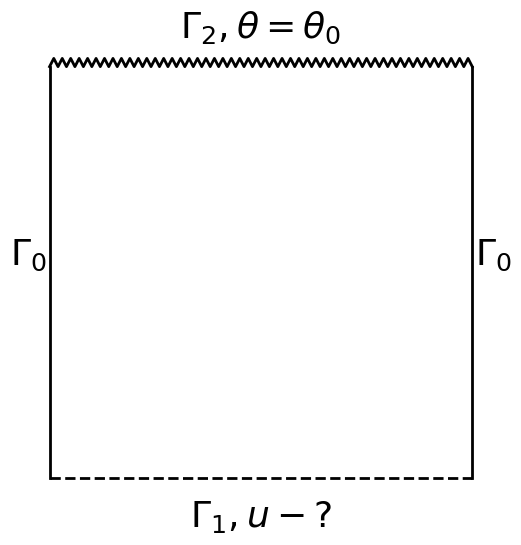
\includegraphics[width=1\linewidth]{omega_1}}
%        \caption*{$\Gamma \coloneqq \partial \Omega =\overline{\Gamma}_0 \cup \overline{\Gamma}_1 \cup \overline{\Gamma}_2$}
    \end{wrapfigure}
    \begin{gather}
        \label{eq:2_1:initial}
        - a \Delta \theta + b \kappa_a(\theta ^ 3 | \theta | - \varphi) = 0, \\
        - \alpha \Delta \varphi + \kappa_a (\varphi - \theta ^3 | \theta |) = 0,
    \end{gather}
    \begin{equation}
        \label{eq:2_1:initial-boundary}
        \begin{aligned}
            \Gamma &: \; a \partial_n \theta + \beta (\theta - \theta _b) = 0, \\
            \Gamma_0 \cup \Gamma_2 &: \; \alpha \partial_n \varphi
            + \gamma(\varphi - \theta_b ^4 ) = 0, \\
            \Gamma_1 &: \; \alpha \partial_n \varphi + u(\varphi - \theta_b ^4 ) = 0. \\
        \end{aligned}
    \end{equation}
    $\Gamma_0, \Gamma_1, \Gamma_2$ не имеют пересечений.

    Функции $\gamma, \theta_b, \beta$ известны.
    \textit{Неизвестная функция $u$ характеризует отражающие свойства участка границы $\Gamma_1$}.
    Предполагается, что $0 < u_1 \leq u \leq u_2$.

    \textbf{Обратная задача} заключается в отыскании тройки $\theta, \varphi, u$
    по дополнительному условию $\theta|_{\Gamma_2} = \theta_0$.

    \textbf{Экстремальная задача} заключается в минимизации функционала
    \begin{equation}
        \label{eq:2_1:quality}
        J(\theta) = \frac{1}{2} \int_{\Gamma_2} (\theta - \theta_0)^2 d\Gamma
    \end{equation}
    на решениях краевой задачи~\eqref{eq:2_1:initial}--\eqref{eq:2_1:initial-boundary}.
\end{frame}
\note{
    Первая из рассматриваемых задач формулируется следующим образом:
    дана некая область омега,
    на части её границы неизвестен параметр среды $u$, характеризирующий отражающие свойства границы.
    Сам параметр выражается как $(\frac{\varepsilon}{2(2-\varepsilon)})$, где $\varepsilon$ меняется в диапазоне от 0 до 1,
    как следствие на сам параметр накладывается ограничение, такое что $u \in [0, 0.5]$.

    Степень черноты не зависит от направления и определяется формулой
    $\varepsilon_\nu(x) = \frac{I_{\nu,\text{исп}}(x)}{I_{b\nu}(T(x))}$, где
    $I_{\nu,\text{исп}}(x)$ -- интенсивность излучения, испускаемого
    поверхностью при температуре $T(x)$~\cite[53]{Ozisik1976}.
    Требуется отыскать тройку: температурное поле,
    поле излучения и неизвестный параметр
    по дополнительной информации о температуре на границе.
    Вопрос о корректности сформулированной обратной задачи является открытым
    (как её решать тоже вопрос открытый).
    Предлагается заменить обратную задачу на задачу
    оптимального управления, которая состоит в
    минимизации функционала~\eqref{eq:2_1:quality}.
    Решение данной экстремальной задачи называется квазирешением обратной задачи.
    Для нахождения квазирешения был разработан оптимизационный численный метод.

    Постоянные $a$ (температуропроводность $м^2/сек$), $b$(коэфициент радиационного переноса) и
    $\alpha$ (Эффективный коэффициентом оптического взаимодействия)
    определяются следующим образом:
    \[
        a = \frac{k}{\rho c_v},\quad b = \frac{4\sigma n^2 T_{\max}^3}{\rho c_v},
        \quad \alpha=\frac{1}{3\kappa - A \kappa_s},
    \]
    где $k$ -- теплопроводность $(Вт/(м \cdot К)=Дж/(м \cdot с \cdot К))$, $c_v$ -- удельная теплоемкость,
    $\rho$ -- плотность,
    $\sigma$ -- постоянная Стефана-Больцмана $(5.67 \cdot 10^{−8} Вт/(м^2 \cdot К^4))$,
    $n$ -- показатель преломления,
    $T_{\max}$ -- максимальная температура в ненормализованной модели,
    $\kappa = \kappa_s + \kappa_a$ -- коэффициент
    полного взаимодействия,
    $\kappa_s$ -- коэффициент рассеяния, $\kappa_a$ -- коэффициент поглощения.
}


\begin{frame}
    \frametitle{Нахождение квазирешения обратной задачи}
    \begin{gather}
        A_1 \theta + b \kappa_a (| \theta | \theta^3 - \varphi) =
        f, A_2 \varphi + \kappa_a (\varphi - |\theta|\theta^3) + F(\varphi, u) = g.
        \label{eq:2_1:weakOperational}\\
        J(\theta) = \frac{1}{2} \int_{\Gamma_2} (\theta - \theta_0)^2 d\Gamma,
        \label{eq:2_1:qualityOperational}\\
        A_1 p_1 + 4 |\hat{\theta}|^3 \kappa_a(b p_1 - p_2) = f_c,
        \;\; (f_c,v) = - \int_{\Gamma_2} (\hat{\theta} - \theta_0) v d\Gamma,
        \label{eq:2_1:theorem_2_eq1}\\
        A_2 p_2 + \kappa_a (p_2-b p_1) = g_c(p_2, \hat{u}),
        \;(g_c(p_2, \hat{u}), v) = -\int_{\Gamma_1} \hat{u} p_2 v d\Gamma,
        \label{eq:2_1:theorem_2_eq2}\\
        \int_{\Gamma_1} p_2 (\hat{\varphi} - \theta_b^4)(u-w) d\Gamma
        \leq 0 \quad \forall w \in U_{ad}. \label{eq:2_1:theorem_2_eq3}
    \end{gather}
    \textbf{Алгоритм градиентного спуска с проекцией}
    \begin{enumerate}
        \item Выбор шага $\lambda$, числа итераций $N$, управления $u_0 \in U_{ad}$
        -- пространство допустимых управлений.
        \item для $k \leftarrow 0,1,2, \ldots, N$ выполнить:
        \begin{itemize}
            \item Для $u_{k}$, вычислить $y_k = \{\theta_k, \varphi_k\}$ из~\eqref{eq:2_1:weakOperational}.
            \item Вычислить значение $J(\theta_k)$ из уравнения~\eqref{eq:2_1:quality}.
            \item Рассчитать $p_k=\{p_{1k},p_{2k}\}$
            из~\eqref{eq:2_1:theorem_2_eq1}--\eqref{eq:2_1:theorem_2_eq2},
            \item Пересчитать управление
            $u_{k+1} = P_{ad}\left[ u_k - \lambda (\varphi_k - \theta_b^4)p_{2k} \right]$.
        \end{itemize}
    \end{enumerate}
\end{frame}
\note{
    Предложенный в работе алгоритм поиска квазирешения обратной задачи основан
    на выведенных условиях оптимальности
    (доказано, что квазирешение должно
    удовлетворять~\eqref{eq:2_1:weakOperational}--\eqref{eq:2_1:theorem_2_eq2}),
    куда входят сопряженные функции для температуры $p_1$ и излучения $p_2$,
    а также связь между сопряженным состоянием и искомым граничным управлением.
    Для компактной записи краевых задач, используется современная операторная форма.
    Система~\eqref{eq:2_1:weakOperational} является операторной записью краевой задачи,
    где $A_{1,2}$ описывают диффузионные члены модели, остальные моделируют граничные условия.
    Уравнения~\eqref{eq:2_1:theorem_2_eq1}--\eqref{eq:2_1:theorem_2_eq2}
    это сопряженная система,
    а вариационное неравенство~\eqref{eq:2_1:theorem_2_eq3}
    устанавливает связь с оптимальным управлением.

    Приведём алгоритм градиентного спуска с проекцией.
    Обратим внимание, что оператор проекции нужен
    из-за начальных ограничений на функцию управления
    (вызванных физичностью параметра, например).

    Отметим, что в силу невыпуклости экстремальной задачи градиентные алгоритмы не обладают
    свойством глобальной сходимости, что служит основой для их критики, зачастую заслуженной.

    Однако свойства диффузионных моделей сложного теплообмена представленные в диссертации
    и правильный выбор шага градиентного метода обеспечивают сходимость для
    рассматриваемых задач.
    Следующие примеры этот факт демонстрируют.
}

\begin{frame}
    \frametitle{Модель управления температурным полем через граничный параметр}
    Положим $\Omega = \{(x,y), 0 \leq x,y \leq 1\}$, $l = 1$ см.
    Граница $\partial\Omega$:
    \[
        \begin{aligned}
            \Gamma_0 & = \{x=\{0,1\}, y \in [0,1]\} \\
            \Gamma_1 & = \{x\in [0,1], y=0\}
            - \text{участок с неизвестными отр. свойствами}, \\
            \Gamma_2 & = \{x \in [0,1], y=1\} - \text{участок наблюдения}.
        \end{aligned}
    \]
    Будем также далее считать, что $a = 0.006[\text{см}^2/\text{c}]$,
    $b=0.025[\text{см}/\text{с}]$, $\beta = 0.00005[\text{см}/\text{с}]$,
    $\kappa=1[\text{см}^{-1}]$, $\kappa_s = 0$, $A = 0$, $\gamma = 0.3$.
    Температуру на границе $\Omega$ положим равной $\theta_b = (x^2+y^2)/3$.

    При указанных параметрах для первого эксперимента выберем следующее тестовое
    значение функции $u$:
    \begin{equation*}
        u(x)=
        \begin{cases}
            0.01, & \text{если } x \le 0.5, \\
            0.5, & \text{если } x > 0.5,
        \end{cases}
    \end{equation*}
    и для второго эксперимента:
    $u(x)=0.49x+0.01$.
\end{frame}
\note{
    Положим параметры среды, соответствующие стеклу и зададим тестовую функцию управления
    как показано на слайде.
    Пластинка, у которого боковые стороны "обычные", верхняя грань - участок наблюдения,
    нижняя грань - участок под "контролем".
}


\begin{frame}
    \frametitle{Модель управления температурным полем через граничные параметр}
    \centering
    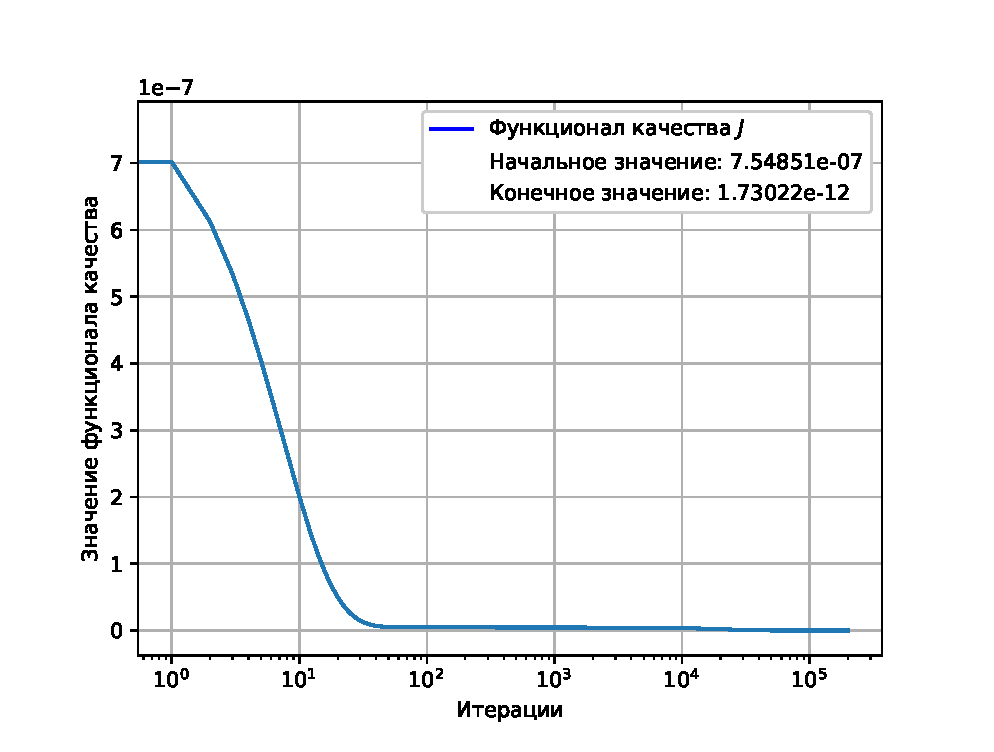
\includegraphics[width=0.495\linewidth]{dvmg368/3}
    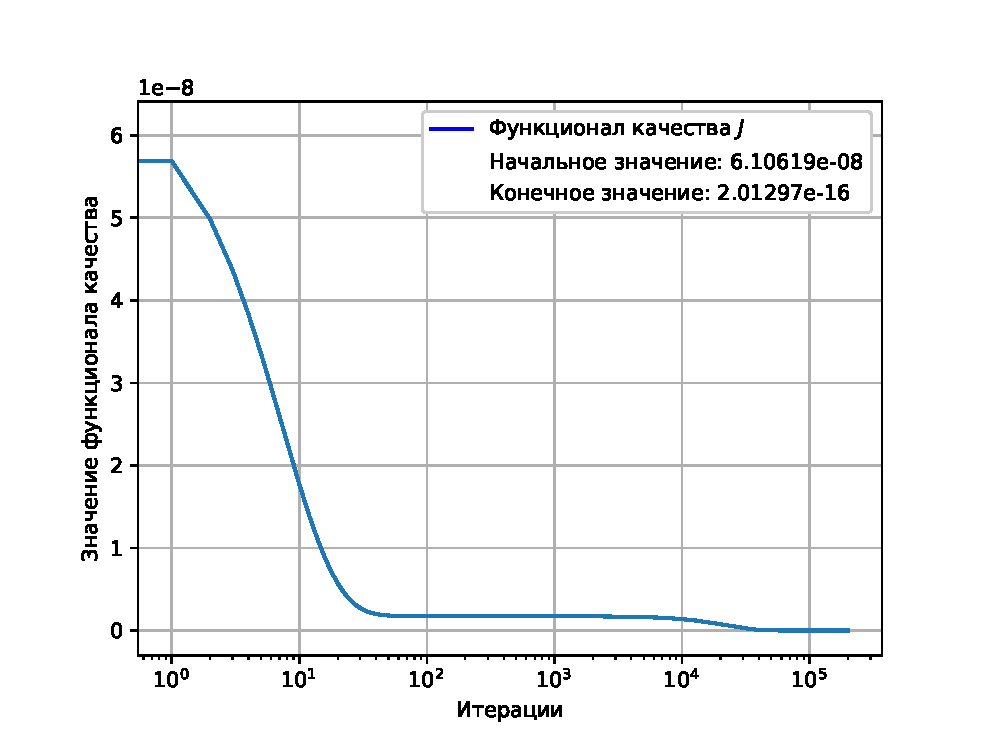
\includegraphics[width=0.495\linewidth]{dvmg368/4}
    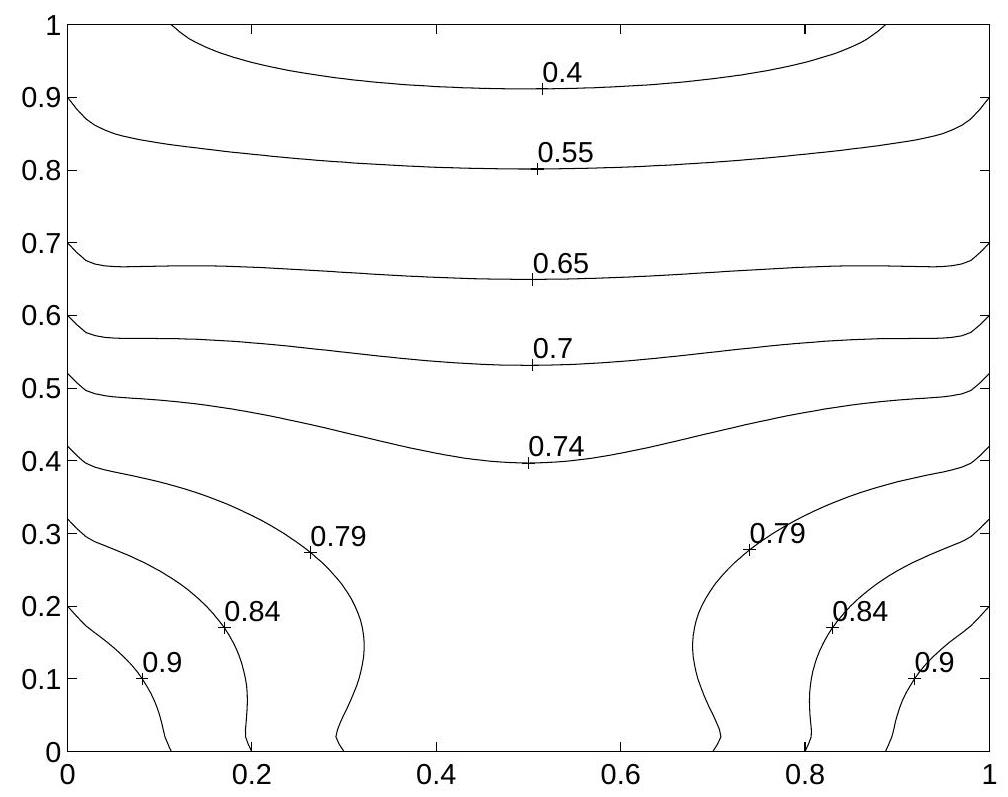
\includegraphics[width=0.495\linewidth]{dvmg368/1}
    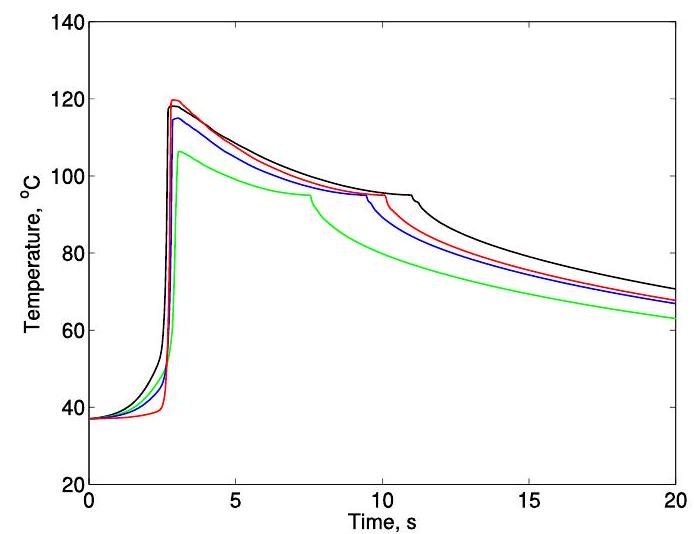
\includegraphics[width=0.495\linewidth]{dvmg368/2}
\end{frame}
\note{
    Интересный эффект "среднего значения". Большое количество итераций.
    Обратить внимание на функционал качества.
    Для получения представленных результатов, использовался разработанный мной комплекс программ,
    включающий решение прямой задачи, сопряженной системы и алгоритм градиентного спуска.
}

\subsection{Обратная задача с условиями типа Коши}\label{subsec:rev_koshi}
\begin{frame}
    \frametitle{Задача без краевых условий для интенсивности излучения}
    \textbf{Краевая задача:}
    \begin{equation}
        \label{eq:2_2:eq1}
        - a \Delta \theta + b \kappa_a(\theta ^ 3 | \theta | - \varphi) = 0,  \quad
        - \alpha \Delta \varphi + \kappa_a (\varphi - \theta ^3 | \theta |) = 0,
    \end{equation}
    На $\Gamma$ известно температурное поле и тепловой поток:
    \begin{equation}
        \label{eq:2_2:bc2} \theta = \theta_b, \quad \partial_n\theta = q_b.
    \end{equation}
    Заменяем на <<искусственные>> краевые условия
    \begin{equation}
        \label{eq:2_2:bc3}
        a(\partial_n\theta+\theta) = r,\;\;
        \alpha(\partial_n\varphi+\varphi) = u \text{ на }\Gamma.
    \end{equation}
    Функция $r(x),\, x\in\Gamma$ является заданной, функция $u(x),\, x\in\Gamma$
    описывающая излучающие свойства участка границы, неизвестна.
    Получаем \textbf{обратную задачу}.

    \textbf{Экстремальная задача} заключается в отыскании тройки
    $\{\theta_\lambda,\varphi_\lambda,u_\lambda\}$ такой, что
    \begin{equation}
        \label{eq:2_2:cost}
        J_\lambda(\theta, u) = \frac{1}{2}\int\limits_\Gamma (\theta - \theta_b)^2 d\Gamma
        + \frac{\lambda}{2}\int\limits_\Gamma u^2 d\Gamma \rightarrow\inf
    \end{equation}
    на решениях краевой задачи, функция $u(x) x \in \Gamma$ играет роль управления.

    \begin{itemize}
        \item $(j) \;\; a,b,\alpha,\kappa_a, \lambda ={\textrm Const}> 0,$
        \item $(jj) \;\, \theta_b, \,q_b \in U,\;\; r=a(\theta_b+q_b)$.
    \end{itemize}
    \begin{theorem}[2.3]
        \label{th:2_2:1}
        Пусть выполняются условия $(j), (jj)$.
        Тогда существует решение экстремальной задачи.
    \end{theorem}
\end{frame}
\note{
    23. Не задано $\varphi$!
    В основе разработанного алгоритма решения лежит анализ экстремальной задачи.

    Строго обосновано существование решения экстр задачи.
    Кроме того, и это принципиально важно, показана сходимость решений экстремальных задач
    к решению задачи~\eqref{eq:2_2:eq1}--\eqref{eq:2_2:eq2}
    без краевых условий для интенс излучения при $\lambda$ стремящемся к 0.
}
\begin{frame}
    \frametitle{Пример 1}
    \textbf{Задача $CP$.} Найти тройку $\{\theta, \varphi, u \} \in V \times V \times U$
    такую, что
    \begin{equation}
        \label{eq:2_2:cp}
        J_\lambda(\theta, u) \equiv \frac{1}{2}\|\theta -\theta_b\|^2_\Gamma
        + \frac{\lambda}{2}\|u\|^2_\Gamma \rightarrow \inf,\;\; F(\theta, \varphi, u)=0.
    \end{equation}
    Для обозначенных параметров рассчитаем функции $\theta$, $\varphi$ из решения граничной задачи
    и положим $\theta_b = \theta|_\Gamma$.
    Нормальная производная $\partial_n \theta = q_b = r / a - \theta_b$.

    Применяя алгоритм градиентного спуска найдем решение задачи $CP$.
    \begin{figure}[h!t]
        \begin{minipage}[b][][b]{0.49\linewidth}
            \centering
            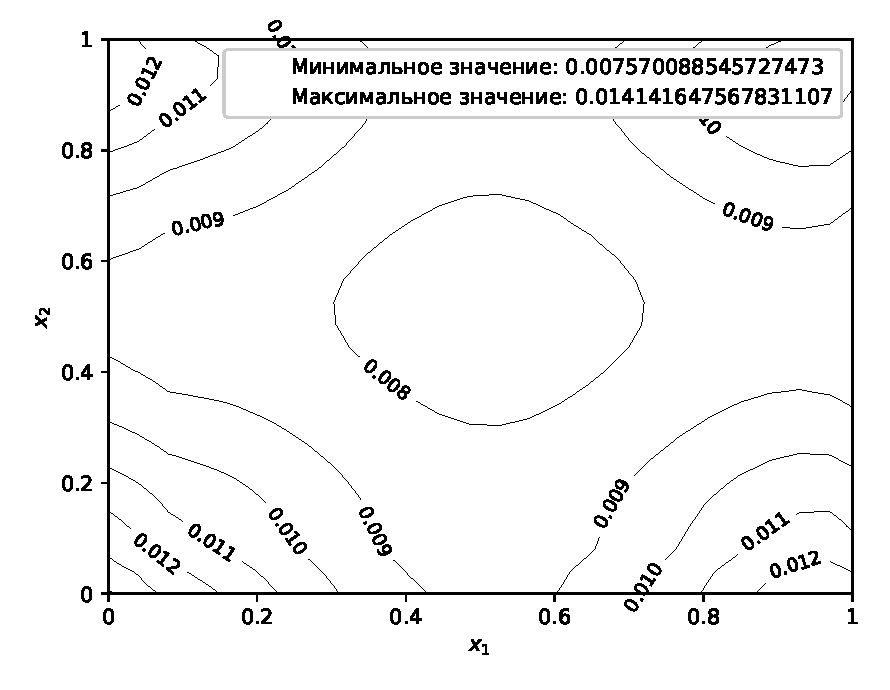
\includegraphics[width=1\linewidth]{jvm-2020/exp1/theta_n_diff_iso}
            \\ а) $|\partial_n\theta_\lambda-q_b|/|q_b|$
        \end{minipage}
        \hfill
        \begin{minipage}[b][][b]{0.49\linewidth}
            \centering
            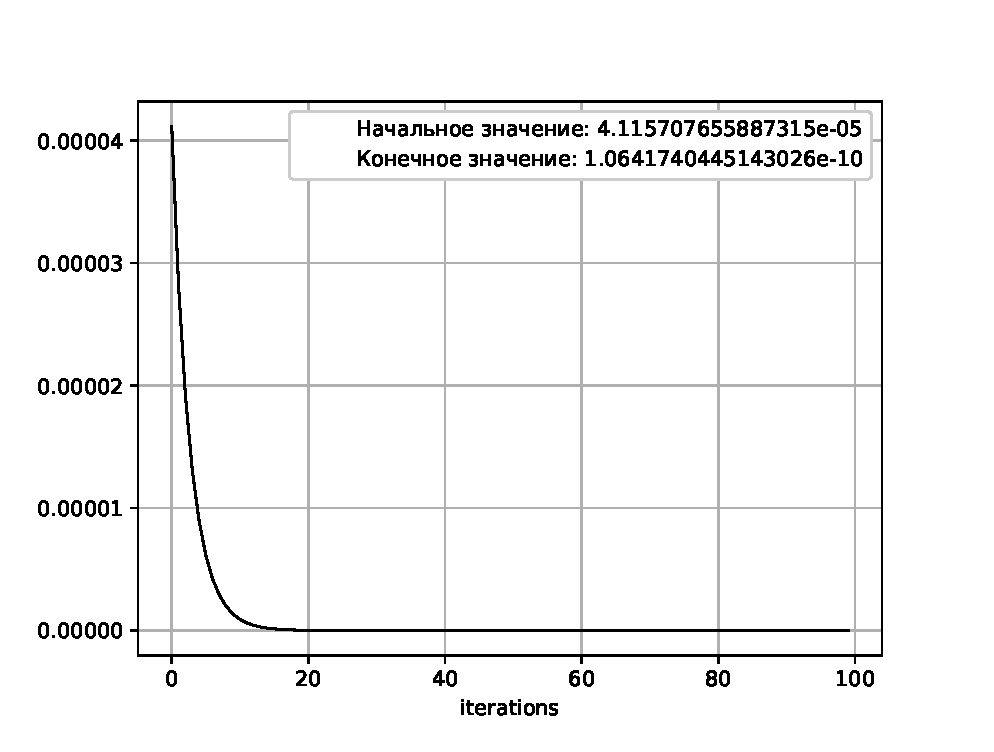
\includegraphics[width=1\linewidth]{jvm-2020/exp1/quality}
            \\ б) Значение функционала качества
        \end{minipage}
        \label{fig:4_4:0}
    \end{figure}
\end{frame}
\note{
    Обратите внимание на малость функционала качества.
    Сравним с тем, что получилось -- довольно близко, но не идеально.
    Уменьшение параметра регуляризации повышает точность решения,
    но и увеличивает вычислительные затраты.
}

\begin{frame}
    \frametitle{Пример 2}
    Зададим функции $\theta_{b}, q_{b}$ в краевом условии~\eqref{eq:2_2:bc2}
    следующим образом:
    \[
        \theta_{b}=0.1 z+0.3, \quad q_{b}=
        \begin{cases}
            0.11, & \text { если } z=1, \\
            0, & \text { если } 0<z<1, \\
            -0.15, & \text { если } z=0.
        \end{cases}
    \]

    В данном примере оптимальное управление $u$ в качестве тестового не задается.

    \begin{figure}[h!t]
        \begin{minipage}[b][][b]{0.49\linewidth}
            \centering
            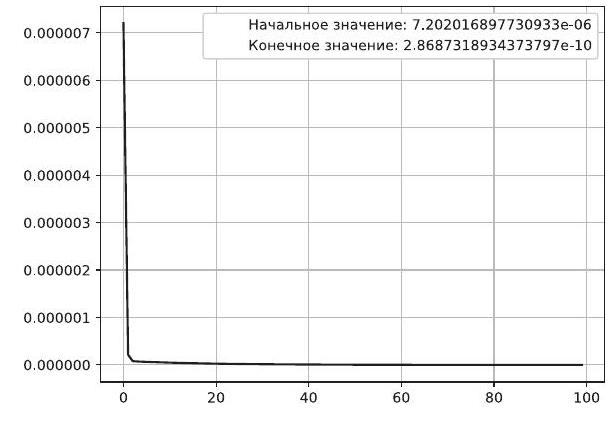
\includegraphics[width=0.9\linewidth]{jvm-2020/dvmg/3a}
            \\ а) Изменение функционала в зависимости от числа итераций
        \end{minipage}
        \hfill
        \begin{minipage}[b][][b]{0.49\linewidth}
            \centering
            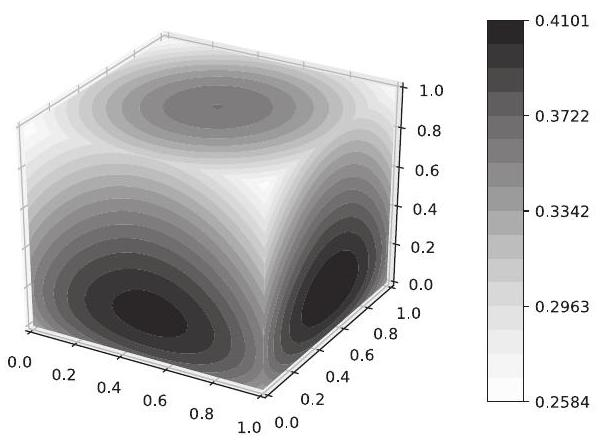
\includegraphics[width=1\linewidth]{jvm-2020/dvmg/2b}
            \\ б) Оптимальное управление
        \end{minipage}
        \label{fig:4_4:3}
    \end{figure}

\end{frame}
\note{
    "Честный" эксперимент - используем то, что полагается в исходной задаче.
    Функционал качества (его динамика) позволяет предположить аналогичный порядок
    близости (с предыдущим примером)
    точного и аппроксимированного решений.
    Обратите внимание на линейность $\theta_b$ по оси $z$.
}
